%%%%%%%%%%%%%%%%%%%%%%%%%%%%%%%%%%%%%%%%%
% Classicthesis Typographic Thesis
% LaTeX Template
% Version 1.1 (4/8/12)
%
% This template has been downloaded from:
% http://www.LaTeXTemplates.com
%
% Original author:
% André Miede (http://www.miede.de)
%
% License:
% CC BY-NC-SA 3.0 (http://creativecommons.org/licenses/by-nc-sa/3.0/)
%
% General Tips:
% 1) Make sure to edit the classicthesis-config.file
% 2) New enumeration (A., B., C., etc in small caps): \begin{aenumerate} \end{aenumerate}
% 3) For margin notes: \marginpar or \graffito{}
% 4) Do not use bold fonts in this style, it is designed around them
% 5) Use tables as in the examples
% 6) See classicthesis-preamble.sty for useful commands
%
%%%%%%%%%%%%%%%%%%%%%%%%%%%%%%%%%%%%%%%%%

%----------------------------------------------------------------------------------------
%	PACKAGES AND OTHER DOCUMENT CONFIGURATIONS
%----------------------------------------------------------------------------------------

\documentclass[
		twoside,openright,titlepage,numbers=noenddot,headinclude,%1headlines,
                footinclude=true,cleardoublepage=empty,
                BCOR=5mm,paper=a4,fontsize=11pt, % Binding correction, paper type and font size
                ngerman,american, % Languages
                ]{scrreprt}

% Includes the file which contains all the document configurations and packages - make sure to edit this file
%%%%%%%%%%%%%%%%%%%%%%%%%%%%%%%%%%%%%%%%%
% Thesis Configuration File
%
% The main lines to change in this file are in the DOCUMENT VARIABLES
% section, the rest of the file is for advanced configuration.
%
%%%%%%%%%%%%%%%%%%%%%%%%%%%%%%%%%%%%%%%%%

%----------------------------------------------------------------------------------------
%	DOCUMENT VARIABLES
%	Fill in the lines below to enter your information into the thesis template
%	Each of the commands can be cited anywhere in the thesis
%----------------------------------------------------------------------------------------

% Remove drafting to get rid of the '[ Date - classicthesis version 4.0 ]' text at the bottom of every page
\PassOptionsToPackage{eulerchapternumbers,listings,drafting,pdfspacing, subfig,beramono,eulermath,parts}{classicthesis}
% Available options: drafting parts nochapters linedheaders eulerchapternumbers beramono eulermath pdfspacing minionprospacing tocaligned dottedtoc manychapters listings floatperchapter subfig
% Adding 'dottedtoc' will make page numbers in the table of contents flushed right with dots leading to them

\newcommand{\myTitle}{3d Plotting Of Aircraft Attitude\xspace}
\newcommand{\mySubtitle}{An Homage to The Elements of Typographic Style\xspace}
\newcommand{\myDegree}{Bachelor of Engineering (Computer Engineering)\xspace}
\newcommand{\myName}{Muhammad Omer Iqbal\xspace}
\newcommand{\myProf}{Put name here\xspace}
\newcommand{\myOtherProf}{Put name here\xspace}
\newcommand{\mySupervisor}{Put name here\xspace}
\newcommand{\myFaculty}{Put data here\xspace}
\newcommand{\myDepartment}{Put data here\xspace}
\newcommand{\myUni}{National University of Singapore\xspace}
\newcommand{\myLocation}{Singapore\xspace}
\newcommand{\myTime}{November 2013\xspace}
\newcommand{\myVersion}{version 2.0\xspace}

%----------------------------------------------------------------------------------------
%	USEFUL COMMANDS
%----------------------------------------------------------------------------------------

\newcommand{\ie}{i.\,e.}
\newcommand{\Ie}{I.\,e.}
\newcommand{\eg}{e.\,g.}
\newcommand{\Eg}{E.\,g.}

\newcounter{dummy} % Necessary for correct hyperlinks (to index, bib, etc.)
\providecommand{\mLyX}{L\kern-.1667em\lower.25em\hbox{Y}\kern-.125emX\@}

%----------------------------------------------------------------------------------------
%	PACKAGES
%----------------------------------------------------------------------------------------

\usepackage{lipsum} % Used for inserting dummy 'Lorem ipsum' text into the template

%------------------------------------------------

\PassOptionsToPackage{latin9}{inputenc} % latin9 (ISO-8859-9) = latin1+"Euro sign"
\usepackage{inputenc}

 %------------------------------------------------

%\PassOptionsToPackage{ngerman,american}{babel}  % Change this to your language(s)
% Spanish languages need extra options in order to work with this template
%\PassOptionsToPackage{spanish,es-lcroman}{babel}
\usepackage{babel}

%------------------------------------------------

\PassOptionsToPackage{square,numbers}{natbib}
 \usepackage{natbib}

 %------------------------------------------------

\PassOptionsToPackage{fleqn}{amsmath} % Math environments and more by the AMS
 \usepackage{amsmath}

 %------------------------------------------------

\PassOptionsToPackage{T1}{fontenc} % T2A for cyrillics
\usepackage{fontenc}

%------------------------------------------------

\usepackage{xspace} % To get the spacing after macros right

%------------------------------------------------

\usepackage{mparhack} % To get marginpar right

%------------------------------------------------

\usepackage{fixltx2e} % Fixes some LaTeX stuff

%------------------------------------------------

\PassOptionsToPackage{smaller}{acronym} % Include printonlyused in the first bracket to only show acronyms used in the text
\usepackage{acronym} % nice macros for handling all acronyms in the thesis

%------------------------------------------------

%\renewcommand*{\acsfont}[1]{\textssc{#1}} % For MinionPro
\renewcommand{\bflabel}[1]{{#1}\hfill} % Fix the list of acronyms

%------------------------------------------------

\PassOptionsToPackage{pdftex}{graphicx}
\usepackage{graphicx}

%----------------------------------------------------------------------------------------
%	FLOATS: TABLES, FIGURES AND CAPTIONS SETUP
%----------------------------------------------------------------------------------------

\usepackage{tabularx} % Better tables
\setlength{\extrarowheight}{3pt} % Increase table row height
\newcommand{\tableheadline}[1]{\multicolumn{1}{c}{\spacedlowsmallcaps{#1}}}
\newcommand{\myfloatalign}{\centering} % To be used with each float for alignment
\usepackage{caption}
\captionsetup{format=hang,font=small}
\usepackage{subfig}

%----------------------------------------------------------------------------------------
%	CODE LISTINGS SETUP
%----------------------------------------------------------------------------------------

\usepackage{listings}
%\lstset{emph={trueIndex,root},emphstyle=\color{BlueViolet}}%\underbar} % for special keywords
\lstset{language=[LaTeX]Tex, % Specify the language for listings here
keywordstyle=\color{RoyalBlue}, % Add \bfseries for bold
basicstyle=\small\ttfamily, % Makes listings a smaller font size and a different font
%identifierstyle=\color{NavyBlue}, % Color of text inside brackets
commentstyle=\color{Green}\ttfamily, % Color of comments
stringstyle=\rmfamily, % Font type to use for strings
numbers=left, % Change left to none to remove line numbers
numberstyle=\scriptsize, % Font size of the line numbers
stepnumber=5, % Increment of line numbers
numbersep=8pt, % Distance of line numbers from code listing
showstringspaces=false, % Sets whether spaces in strings should appear underlined
breaklines=true, % Force the code to stay in the confines of the listing box
%frameround=ftff, % Uncomment for rounded frame
frame=single, % Frame border - none/leftline/topline/bottomline/lines/single/shadowbox/L
belowcaptionskip=.75\baselineskip % Space after the "Listing #: Desciption" text and the listing box
}

%----------------------------------------------------------------------------------------
%	HYPERREFERENCES
%----------------------------------------------------------------------------------------

\PassOptionsToPackage{pdftex,hyperfootnotes=false,pdfpagelabels}{hyperref}
\usepackage{hyperref}  % backref linktocpage pagebackref
\pdfcompresslevel=9
\pdfadjustspacing=1

\hypersetup{
% Uncomment the line below to remove all links (to references, figures, tables, etc)
%draft,
colorlinks=true, linktocpage=true, pdfstartpage=3, pdfstartview=FitV,
% Uncomment the line below if you want to have black links (e.g. for printing black and white)
%colorlinks=false, linktocpage=false, pdfborder={0 0 0}, pdfstartpage=3, pdfstartview=FitV,
breaklinks=true, pdfpagemode=UseNone, pageanchor=true, pdfpagemode=UseOutlines,
plainpages=false, bookmarksnumbered, bookmarksopen=true, bookmarksopenlevel=1,
hypertexnames=true, pdfhighlight=/O, urlcolor=webbrown, linkcolor=RoyalBlue, citecolor=webgreen,
%------------------------------------------------
% PDF file meta-information
pdftitle={\myTitle},
pdfauthor={\textcopyright\ \myName, \myUni, \myFaculty},
pdfsubject={},
pdfkeywords={},
pdfcreator={pdfLaTeX},
pdfproducer={LaTeX with hyperref and classicthesis}
%------------------------------------------------
}

%----------------------------------------------------------------------------------------
%	BACKREFERENCES
%----------------------------------------------------------------------------------------

\usepackage{ifthen} % Allows the user of the \ifthenelse command
\newboolean{enable-backrefs} % Variable to enable backrefs in the bibliography
\setboolean{enable-backrefs}{false} % Variable value: true or false

\newcommand{\backrefnotcitedstring}{\relax} % (Not cited.)
\newcommand{\backrefcitedsinglestring}[1]{(Cited on page~#1.)}
\newcommand{\backrefcitedmultistring}[1]{(Cited on pages~#1.)}
\ifthenelse{\boolean{enable-backrefs}} % If backrefs were enabled
{
\PassOptionsToPackage{hyperpageref}{backref}
\usepackage{backref} % to be loaded after hyperref package
\renewcommand{\backreftwosep}{ and~} % separate 2 pages
\renewcommand{\backreflastsep}{, and~} % separate last of longer list
\renewcommand*{\backref}[1]{}  % disable standard
\renewcommand*{\backrefalt}[4]{% detailed backref
\ifcase #1
\backrefnotcitedstring
\or
\backrefcitedsinglestring{#2}
\else
\backrefcitedmultistring{#2}
\fi}
}{\relax}

%----------------------------------------------------------------------------------------
%	AUTOREFERENCES SETUP
%	Redefines how references in text are prefaced for different
%	languages (e.g. "Section 1.2" or "section 1.2")
%----------------------------------------------------------------------------------------

\makeatletter
\@ifpackageloaded{babel}
{
\addto\extrasamerican{
\renewcommand*{\figureautorefname}{Figure}
\renewcommand*{\tableautorefname}{Table}
\renewcommand*{\partautorefname}{Part}
\renewcommand*{\chapterautorefname}{Chapter}
\renewcommand*{\sectionautorefname}{Section}
\renewcommand*{\subsectionautorefname}{Section}
\renewcommand*{\subsubsectionautorefname}{Section}
}
\addto\extrasngerman{
\renewcommand*{\paragraphautorefname}{Absatz}
\renewcommand*{\subparagraphautorefname}{Unterabsatz}
\renewcommand*{\footnoteautorefname}{Fu\"snote}
\renewcommand*{\FancyVerbLineautorefname}{Zeile}
\renewcommand*{\theoremautorefname}{Theorem}
\renewcommand*{\appendixautorefname}{Anhang}
\renewcommand*{\equationautorefname}{Gleichung}
\renewcommand*{\itemautorefname}{Punkt}
}
\providecommand{\subfigureautorefname}{\figureautorefname} % Fix to getting autorefs for subfigures right
}{\relax}
\makeatother

%----------------------------------------------------------------------------------------

\usepackage{classicthesis}

%----------------------------------------------------------------------------------------
%	CHANGING TEXT AREA
%----------------------------------------------------------------------------------------

%\linespread{1.05} % a bit more for Palatino
%\areaset[current]{312pt}{761pt} % 686 (factor 2.2) + 33 head + 42 head \the\footskip
%\setlength{\marginparwidth}{7em}%
%\setlength{\marginparsep}{2em}%

%----------------------------------------------------------------------------------------
%	USING DIFFERENT FONTS
%----------------------------------------------------------------------------------------

%\usepackage[oldstylenums]{kpfonts} % oldstyle notextcomp
%\usepackage[osf]{libertine}
%\usepackage{hfoldsty} % Computer Modern with osf
%\usepackage[light,condensed,math]{iwona}
%\renewcommand{\sfdefault}{iwona}
%\usepackage{lmodern} % <-- no osf support :-(
%\usepackage[urw-garamond]{mathdesign} <-- no osf support :-(

\usepackage{listings}
\usepackage{color}

\definecolor{dkgreen}{rgb}{0,0.6,0}
\definecolor{gray}{rgb}{0.5,0.5,0.5}
\definecolor{mauve}{rgb}{0.58,0,0.82}

\lstset{frame=tb,
  language=Lisp,
  aboveskip=3mm,
  belowskip=3mm,
  showstringspaces=false,
  columns=flexible,
  basicstyle={\small\ttfamily},
  numbers=none,
  numberstyle=\tiny\color{gray},
  keywordstyle=\color{blue},
  commentstyle=\color{dkgreen},
  stringstyle=\color{mauve},
  breaklines=true,
  breakatwhitespace=true
  tabsize=3
}


\begin{document}

\frenchspacing % Reduces space after periods to make text more compact

\raggedbottom % Makes all pages the height of the text on that page

\selectlanguage{american} % Select your default language - e.g. american or ngerman

%\renewcommand*{\bibname}{new name} % Uncomment to change the name of the bibliography
%\setbibpreamble{} % Uncomment to include a preamble to the bibliography - some text before the reference list starts

\pagenumbering{roman} % Roman page numbering prior to the start of the thesis content (i, ii, iii, etc)

\pagestyle{plain} % Suppress headers for the pre-content pages

%----------------------------------------------------------------------------------------
%	PRE-CONTENT THESIS PAGES
%----------------------------------------------------------------------------------------

% Title Page

\begin{titlepage}

\begin{addmargin}[-1cm]{-3cm}

\begin{center}
\large

\hfill

\vfill

B.Eng. Dissertation \\ \bigskip \bigskip

\begingroup
\color{Maroon}\spacedallcaps{\myTitle} \\ \bigskip % Thesis title
\endgroup

by \\
\spacedlowsmallcaps{\myName}
\\ % Your name
\bigskip
\myUni\\
\myYear
\bigskip
\vfill

%
\includegraphics[width=6cm]{gfx/TFZsuperellipse_bw} \\ \medskip % Picture

{\raggedright Project ID: \myProjId\\
Project Supervisor: \mySupervisor\\
Deliverables: \\
Report: 1 Volume \\
}
%\mySubtitle \\ \medskip % Thesis subtitle
%\myDegree \\
%\myDepartment \\
%\myFaculty \\
%\myUni \\ \bigskip

%\myTime\ -- \myVersion % Time and version

\vfill

\end{center}
\end{addmargin}

\end{titlepage}
 % Main title page

% Back of the title page

\thispagestyle{empty}

\hfill

\vfill

\noindent\myName: \textit{\myTitle,} \myDegree,
\textcopyright\ \myTime

% You may wish to do something with the back of the title page, such as including your supervisors, location or time frame of the work. Below is an example of doing so although you may want to tweak it to your liking.

%\bigskip

%\noindent\spacedlowsmallcaps{Supervisors}: \\
%\myProf \\
%\myOtherProf \\
%\mySupervisor

%\medskip \\

%\noindent\spacedlowsmallcaps{Location}: \\
%\myLocation

%\medskip \\

%\noindent\spacedlowsmallcaps{Time Frame}: \\
%\myTime
 % Back of the title page

%\cleardoublepage% Dedication

\thispagestyle{empty}
\refstepcounter{dummy}

\pdfbookmark[1]{Dedication}{Dedication} % Bookmark name visible in a PDF viewer

\vspace*{3cm}

\begin{center}
\emph{Ohana} means family. \\
Family means nobody gets left behind, or forgotten. \\ \medskip
--- Lilo \& Stitch    
\end{center}

\medskip

\begin{center}
Dedicated to the loving memory of Rudolf Miede. \\ \smallskip
1939\,--\,2005
\end{center} % Dedication page

%\cleardoublepage\include{FrontBackMatter/Foreword} % Uncomment and create a Foreword.tex to include a foreword

\cleardoublepage% Abstract

\pdfbookmark[1]{Abstract}{Abstract} % Bookmark name visible in a PDF viewer

\begingroup
\let\clearpage\relax
\let\cleardoublepage\relax
\let\cleardoublepage\relax

\chapter*{Abstract} % Abstract name

Short summary of the contents\dots

\endgroup			

\vfill % Abstract page

%\cleardoublepage% Publications - a page listing research articles written using content in the thesis

\pdfbookmark[1]{Publications}{Publications} % Bookmark name visible in a PDF viewer

\chapter*{Publications} % Publications page text

Some ideas and figures have appeared previously in the following publications:

\bigskip

\noindent Put your publications from the thesis here. The packages \texttt{multibib} or \texttt{bibtopic} etc. can be used to handle multiple different bibliographies in your document. % Publications from the thesis page

\cleardoublepage% Acknowledgements

\pdfbookmark[1]{Acknowledgements}{Acknowledgements} % Bookmark name visible in a PDF viewer

\begin{flushright}{\slshape    
We have seen that computer programming is an art, \\ 
because it applies accumulated knowledge to the world, \\ 
because it requires skill and ingenuity, and especially \\
because it produces objects of beauty.} \\ \medskip
--- \defcitealias{knuth:1974}{Donald E. Knuth}\citetalias{knuth:1974} \citep{knuth:1974}
\end{flushright}

\bigskip

%----------------------------------------------------------------------------------------

\begingroup

\let\clearpage\relax
\let\cleardoublepage\relax
\let\cleardoublepage\relax

\chapter*{Acknowledgements} % Acknowledgements section text

Put your acknowledgements here.\\

\noindent Many thanks to everybody who already sent me a postcard!\\

\noindent Regarding the typography and other help, many thanks go to Marco Kuhlmann, Philipp Lehman, Lothar Schlesier, Jim Young, Lorenzo Pantieri and Enrico Gregorio\footnote{Members of GuIT (Gruppo Italiano Utilizzatori di \TeX\ e \LaTeX )}, J\"org Sommer, Joachim K\"ostler, Daniel Gottschlag, Denis Aydin, Paride Legovini, Steffen Prochnow, Nicolas Repp, Hinrich Harms, Roland Winkler,  and the whole \LaTeX-community for support, ideas and some great software.

\bigskip

\noindent\emph{Regarding \mLyX}: The \mLyX\ port was intially done by
\emph{Nicholas Mariette} in March 2009 and continued by
\emph{Ivo Pletikosi\'c} in 2011. Thank you very much for your work and the contributions to the original style.

\endgroup % Acknowledgements page

\pagestyle{scrheadings} % Show chapter titles as headings

\cleardoublepage% Table of Contents - List of Tables/Figures/Listings and Acronyms

\refstepcounter{dummy}

\pdfbookmark[1]{\contentsname}{tableofcontents} % Bookmark name visible in a PDF viewer

\setcounter{tocdepth}{2} % Depth of sections to include in the table of contents - currently up to subsections

\setcounter{secnumdepth}{3} % Depth of sections to number in the text itself - currently up to subsubsections

\manualmark
\markboth{\spacedlowsmallcaps{\contentsname}}{\spacedlowsmallcaps{\contentsname}}
\tableofcontents
\automark[section]{chapter}
\renewcommand{\chaptermark}[1]{\markboth{\spacedlowsmallcaps{#1}}{\spacedlowsmallcaps{#1}}}
\renewcommand{\sectionmark}[1]{\markright{\thesection\enspace\spacedlowsmallcaps{#1}}}

\clearpage

\begingroup
\let\clearpage\relax
\let\cleardoublepage\relax
\let\cleardoublepage\relax

%----------------------------------------------------------------------------------------
%	List of Figures
%----------------------------------------------------------------------------------------

\refstepcounter{dummy}
%\addcontentsline{toc}{chapter}{\listfigurename} % Uncomment if you would like the list of figures to appear in the table of contents
\pdfbookmark[1]{\listfigurename}{lof} % Bookmark name visible in a PDF viewer

\listoffigures

\vspace*{8ex}
\newpage

%----------------------------------------------------------------------------------------
%	List of Tables
%----------------------------------------------------------------------------------------

%\refstepcounter{dummy}
%\addcontentsline{toc}{chapter}{\listtablename} % Uncomment if you would like the list of tables to appear in the table of contents
%\pdfbookmark[1]{\listtablename}{lot} % Bookmark name visible in a PDF viewer

%\listoftables

%\vspace*{8ex}
%\newpage

%----------------------------------------------------------------------------------------
%	List of Listings
%----------------------------------------------------------------------------------------

\refstepcounter{dummy}
%\addcontentsline{toc}{chapter}{\lstlistlistingname} % Uncomment if you would like the list of listings to appear in the table of contents
\pdfbookmark[1]{\lstlistlistingname}{lol} % Bookmark name visible in a PDF viewer

\lstlistoflistings

\vspace*{8ex}
\newpage

%----------------------------------------------------------------------------------------
%	Acronyms
%----------------------------------------------------------------------------------------

\refstepcounter{dummy}
%\addcontentsline{toc}{chapter}{Acronyms} % Uncomment if you would like the acronyms to appear in the table of contents
\pdfbookmark[1]{Acronyms}{acronyms} % Bookmark name visible in a PDF viewer

\markboth{\spacedlowsmallcaps{Acronyms}}{\spacedlowsmallcaps{Acronyms}}

\chapter*{Acronyms}

\begin{acronym}[UML]
\acro{DRY}{Don't Repeat Yourself}
\acro{API}{Application Programming Interface}
\acro{UML}{Unified Modeling Language}
\acro{KML}{Keyhole Markup Language}
\acro{AAIB}{Air Accident Investigation Board}
\acro{DOM}{Document Object Model}
\acro{REPL}{Read Eval Print Loop}
\end{acronym}

\endgroup

\cleardoublepage
 % Contents, list of figures/tables/listings and acronyms

\pagenumbering{arabic} % Arabic page numbering for thesis content (1, 2, 3, etc)
%\setcounter{page}{90} % Uncomment to manually start the page counter at an arbitrary value (for example if you wish to count the pre-content pages in the page count)

\cleardoublepage % Avoids problems with pdfbookmark

%----------------------------------------------------------------------------------------
%	THESIS CONTENT - CHAPTERS
%----------------------------------------------------------------------------------------

%\ctparttext{You can put some informational part preamble text here. Illo principalmente su nos. Non message \emph{occidental} angloromanic da. Debitas effortio simplificate sia se, auxiliar summarios da que, se avantiate publicationes via. Pan in terra summarios, capital interlingua se que. Al via multo esser specimen, campo responder que da. Le usate medical addresses pro, europa origine sanctificate nos se.} % Text on the Part 1 page describing  the content in Part 1

\part{The Problem} % First part of the thesis

% Chapter 1

\chapter{Introduction} % Chapter title

\label{ch:introduction} % For referencing the chapter elsewhere, use \autoref{ch:introduction}

%----------------------------------------------------------------------------------------
\section{Background}

Aircraft systems record large quantities of data during flight. A lot of this data is necessary in the system 's proper functioning. It takes an even more significant role when investigating air accidents.
As this data establishes the causes behind those accidents, it aids measures to prevent such accidents from occurring. That is the primary reason for why recovery of Flight Data Recorders \footnote{Popularly referred to as `Blackboxes`} is usually a very high priority for aircraft investigations \citep{faa:fdr}.\\

The data itself features many components tracked over time, including but not limited to the following\footnote{The following components were part of the sample dataset I was given for testing.}:
\begin{itemize}
\item Latitude
\item Longtitude
\item Altitude
\item Heading
\item Pitch
\item Roll
\item Engine Thrust
\item Throttle Lever Position
\end{itemize}

As is probably evident, analyzing this largely numeric data by itself would be a painstaking task. Primarily because finding patterns in numbers through observation is inherently difficult. Also because the data set is of a substantially large size \footnote{I will be cautious before calling it ``Big Data''. }. \\

Therefore the need for a tool to visualise this data becomes immediately obvious. \\

The Air Accident Investigation Board (AAIB), a branch of Singapore's Ministry of Transport performs analysis on such flight data, and requested an application that would render relevant flight data quickly and in a portable manner. \\

\section{System Requirements}

AAIB needed the application to meet certain criterias and contain certain core features. These included:

\begin{enumerate}
  \item \spacedlowsmallcaps{Google Earth} Compatibility. Google Earth is a popular virtual globe, map and geographic information program \citep{google:earth}. It provides detailed 3d projections of Google's satellite images on a spherical globe, overlaid with huge quantities of textual and pictorial data varying from international boundaries to streets. There are many good reasons for this requirement including:
    \begin{itemize}
      \item Cross Platform. It works and is supported on Windows, OSX and Linux \footnote{Atleast the desktop version is supported on all three major Operating Systems.}
      \item Extensible through the Keyhole Markup Language (KML) \footnote{A lot more on this later}
      \item Free\footnote{As in beer, not speech. Though they actually have a paid version with more features}
      \item AAIB's familiarity with it
      \item Offline use. This is quite important as internet access is not guranteed on accident sites
    \end{itemize}
  \item \spacedlowsmallcaps{CSV}\footnote{Comma Separated Values} based input. The system should be able to use large datasets encoded in CSV.
  \item  The system should display the data in its geographical location as vectors. The visualization should be able to reflect the actual data in an intuitive way. For instance, vectors at each data point should represent roll, heading, engine throttle
  \item Users should be able to select which vectors they want to view.
  \item The data points should be manually adjustable from within google earth. This is particularly relevant for data points near landing strips, where measurement errors may cause an offset in the rendered visualization

\end{enumerate}
 % Chapter 1

%\cleardoublepage % Empty page before the start of the next part

%------------------------------------------------

%\ctparttext{You can put some informational part preamble text here. Illo principalmente su nos. Non message \emph{occidental} angloromanic da. Debitas effortio simplificate sia se, auxiliar summarios da que, se avantiate publicationes via. Pan in terra summarios, capital interlingua se que. Al via multo esser specimen, campo responder que da. Le usate medical addresses pro, europa origine sanctificate nos se.} % Text on the Part 2 page describing the content in Part 2

\part{Designing a Solution} % Second part of the thesis

% Chapter 2

\chapter{Rendering Strategies} % Chapter title

\label{ch:rendering strategies} % For referencing the chapter elsewhere, use \autoref{ch:examples}

As with any project, the first few stages of the project involved researching on existing technologies that either implemented the features specified in by AAIB in their requirements, or aided in developing those features. As Google Earth compatibility was a major requirement for the project, my research started with exploring
methods to render custom data on Google Earth's platform.


\section{Keyhole Markup Language}

The Keyhole Markup Language (\emph{KML}) is a subset of XML, used to display geographic data in an Earth Browser, like Google Earth. It uses a tag based structure with nested elements that represent certain geometric
and descriptive constructs \citep{google:kml}. The KML reference is very reasonably documented with sample code demonstrating it's usage.\\

KML supports rendering the following features:
\begin{enumerate}
  \item Placemarks
  \item Descriptions
  \item Ground Overlays
  \item Paths
  \item Polygons
\end{enumerate}

KML uses latitudes and longtitudes as a coordinate system for positioning elements, which works very well with geographic data. \\
However KML is primarily designed as a means to display data, as opposed to performing interactions with the data. The only interactions it allows are those that Google Earth features, i.e. zooming, panning and moving to a certain point on the globe. Clicking on placemarks with descriptions opens a modal that renders the description, which can be written in a subset of HTML. \\

\section{Google Earth's Browser Plugin}

With web browsers becoming increasingly powerful and technologies like WebGL that allow efficient 3d rendering on the browser, Google launched the Google Earth Browser Plugin\citep{google:browser-plugin}. The browser plugin by itself allows pretty much the similar core functionality as Google Earth's Desktop Application. The primary difference is that the virtual globe can be embedded within an HTML web page.\\

By itself the browser plugin may not seem to accomplish much. However Google also released the Google Earth
API, a javascript library that provides access to various features in Google Earth. The browser plugin when combined with Google Earth's API becomes a very powerful tool to produce complex applications that render and allow interaction with geographic data. \\

For instance one of the sample toy applications provided as documentation for the API is a car simulator,
where you drive a car over the virtual globe's surface \citep{google:earth-api}. \\

Such user interactions are possible by combining interactions provided by the DOM, and using them to render models using the Google Earth API. \\

However, the browser plugin is not a silver bullet. One of it's most lacking features is offline usage. The browser plugin does not work offline, unlike the desktop application which caches data for offline use.


\section{Choosing a rendering strategy}

After researching on rendering methods available I had to choose which method was a better fit for this project. From my research the following rendering strategies seemed initially viable:

\begin{enumerate}
\item Generate KML and use it's Path and Polygon constructs to render the various vectors that AAIB requested
\item Use Google Earth's javascript API to render the same data.
\end{enumerate}

After revisiting AAIB's application requirements, I decided that between producing KML and using Google Earth
s Browser Plugin, generating KML was a significantly better option. The rationale guiding the decision was based on the following factors:

\begin{itemize}
\item Offline usage. As mentioned before, the browser plugin does not feature offline usage. This is in contrast to rendering KML documents on Google Earth's Desktop client which works well offline. Considering offline usage was an important part of the application requirements, this was a major reason.
\item Portability. KML is a well defined format that can be rendered on many other earth browsers. Furthermore, the browser plugin is only supported for Windows and Mac OS\citep{google:browser-plugin}. Linux \footnote{Which I am a huge fan of} was not yet supported, and I did not want to add that constraint to the application without good reason. In contrast, Google Earth is supported on Windows, Mac OS and Linux.
\end{itemize}
 % Chapter 2
% Chapter 3

\chapter{Choosing the stack} % Chapter title

\label{ch:stack} % For referencing the chapter elsewhere, use \autoref{ch:mathtest}

This decision took a while. And rightfully so, as it would affect all decisions from that point. Choosing the right language and framework could have more than substantial effects on the system's architecture.\\

After quite a bit of research and debate, I decided to implement the system using \spacedlowsmallcaps{clojure}, a relatively new lisp class language than runs on the JVM.

\section{Clojure?}

The choice of implementing this project in clojure may seem peculiar. However there are a number of features that clojure and it's ecosystem that fit very well with this particular project. Before jumping to those features, a quick overview of clojure is in order.\\

Clojure is a lisp dialect, created by Rich Hickey. It is a general-purpose, functional programming language that runs on the Java Virtual Machine (JVM) \footnote{Clojure runs in other environments like Microsoft's Common Language Runtime (CLR) and Javascript engines as well}. Clojure focuses on programming with immutable data structures and provides a number of persistent hash-trie based data structures that allow efficient functional programming.\\

Clojure was designed to be a real world language, as opposed to a purely academic one.
 % Chapter 3
% Chapter 4

\chapter{Modelling The Problem} % Chapter title

\label{ch:model} % For referencing the chapter elsewhere, use \autoref{ch:name}

As mentioned before, the core function of the application was to convert periodic flight data into a
renderable 3d model. This section will detail the approach taken to model the various aspects of the flight data.\\


\section{Inputs}

As mentioned before

\section{Constraints}

A constraint that choosing KML placed on the model was that any coordinate could only be represented withe following dimensions:
\begin{enumerate}
\item Latitude ($\phi$)
\item Longtitude ($\lambda$)
\item Altitude (a)
\end{enumerate}

This implied that plotting polygons with KML would require converting to and fro between cartesian and spherical coordinate systems.
%----------------------------------------------------------------------------------------

\section{Flight Path}

Plotting the flight path is the most straightforward

%------------------------------------------------

\subsection{Subsection Title}

Content

%------------------------------------------------

\subsection{Subsection Title}

Content

%----------------------------------------------------------------------------------------

\section{Section Title}

Content


\part{Developing the Solution}
%%% Local Variables:
%%% mode: latex
%%% TeX-master: t
%%% End:

\chapter{Implementation}

\label{ch:implementation}

\section{Architecture}

\begin{figure}[h]
\centering
  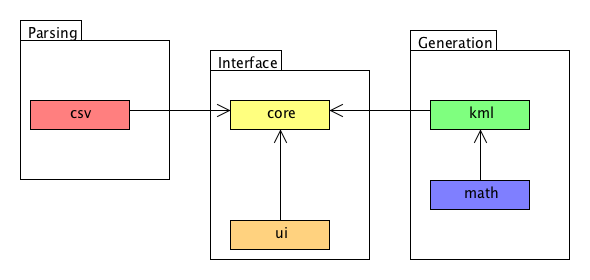
\includegraphics[scale=0.5]{gfx/fyp-arch.png}
\caption{Application architecture as a dependency graph}
\end{figure}

The application was divided into 5 main modules, or namespaces in clojure speak, with each namespace containing functions that perform a particular task. \\

As evident by the figure above, these namespaces were grouped into three broad areas; parsing, interfacing and generation. The primary motivation for having all this classification was to maintain decoupled code. The modularity also helped with keeping the code easier to extend. \\

For example, if the input format was to change, the only module effected would be the csv module. The kml, math and ui namespaces would be unaffected by this change. \\

Another broad aspect of the architecture was to keep the interfaces between the modules well defined. Therefore even though the implementation might change, things would not break.\\

\section{Parsing}

As mentioned in the requirements, the application should be able to read input from a csv file. Parsing the data by itself was pretty straightforward. Clojure comes with a very performant csv parser called clojure.data.csv which returns a sequence of vectors, representing the columns and rows in the csv data set. \\

The parser does need logic to ignore comments, as clojure.data.csv does not recognize them. Nor does it ignore whitespace. Therefore I needed to add some simple logic to filter out whitespace and comments. \\

A very important part of the dataset is the data header. This usually is the first line of the file, if whitespace and comments are ignored. The header specifies which column represents what data. \\

Therefore the csv namespace offers a function called \lstinline{read} which takes a string or a buffered reader, performs the parsing and returns a vector of hash-maps. Each hash-map represents a row, and each value in hash-map represents the value at that row for a particular column. The column names are kept as keys during this representation. \\

As the mapping between column names in the data set and what they represent in the application is not fixed,it would not be wise to hardcode that mapping in the application. The CSV file has no gurantees that the headers would remain the same for all datasets.\\

\begin{lstlisting}[caption= A sample header from the csv dataset]
"Time","Magnetic Heading (DEGS)","Pressure Altitude (feet)","GPS Latitude (degs)","GPS Longitude (degs)","AIR GROUND (0-AIR,1-GND)","Throttle Lever Position Engine 1 (DEGS)","Throttle Lever Position Engine 2 (DEGS)","Throttle Lever Position Engine 3 (DEGS)","Throttle Lever Position Engine 4 (DEGS)","Roll Angle (DEGS)","Pitch Angle (DEGS)","N1 Actual Engine 1 (\%)","N1 Actual Engine 2 (\%)","N1 Actual Engine 3 (\%)","N1 Actual Engine 4 (\%)","UTC Time  (hh:mm:ss)"
\end{lstlisting}

The application tackles this problem in two ways:
\begin{enumerate}

\item The user interface requests the user to fill in the mapping (see figure below).
\item The parser guesses which headers strings correspond to what data. The guessing logic for now is very simple. It simply checks if a field in the header contains a certain substring which would recognize that field. This is not a fool proof method by any means, but helps in reducing work for the user by auto filling the mapping section in the user interface.
\end{enumerate}

To perform the guessing, the csv namespace exposes a function called \lstinline{analyze-headers!}\\

\begin{figure}[h]
\centering
  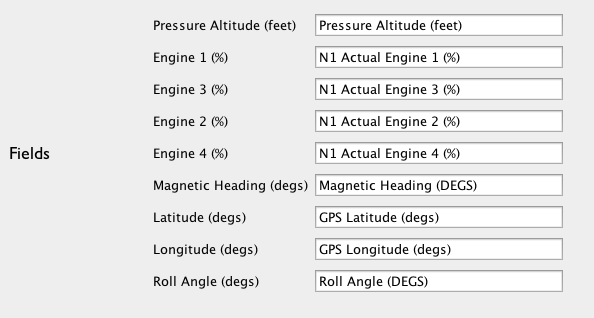
\includegraphics[scale=0.7]{gfx/ui-fields.png}
\caption{User interface allows users to specify field names in the csv file}
\end{figure}

As clojure sequences are lazy data structures, I do not need to worry about heap overflows, if the data size increases. That is the fundamental reason why clojure.data.csv returns a sequence of rows, intead of a vector, which is not lazy.\\

\section{Generation}

There are two main namespaces that classify within generation.

\subsection{math}

As should be evident by the name, this namespace largely implements the mathematical models mentioned in the previous chapter. The main functions it exposes include \lstinline{right-rect-from-edge} and \lstinline{left-rect-from-edge}. \\

\lstinline{left-rect-from-edge} takes a point, width, height, heading and roll angle to produce a rectangle that represents the left wing of an aircraft\footnote{When viewed from behind}. Similarly \lstinline{right-rect-from-edge} does pretty much the same thing for the right wing of the aircraft.\\


\subsection{kml}

This namespace contains functions that do the bulk of the KML generation. The main interface here is the \lstinline{render} function which generates the KML document and emits the result to a file. \\

The hiccup DSL is used very heavily here, along with clojure.data.xml for speedy emission. Hiccup is primarily used to build base XML components which are fed coordinates from calling functions from the  \lstinline{math} namespace. \\

 KML allows specifying styles to elements, which works like a bit like CSS. KML elements can have ids, which Style objects can refer to when they specify styles like line and fill color. Because user's would want the ability to customize colors, the \lstinline{render} function also takes a style configuration as an argument. \\

AAIB also specified in the user requirements, that users should be able to select and unselect various elemnts in the visualisation. This taken care of within this namespace through using KML's Folders to structure the document in a user friendly way. \\

\begin{figure}[h]
\centering
  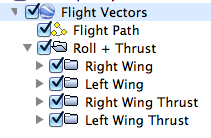
\includegraphics[scale=1]{gfx/kml-structure.png}
\caption{Users can select which components they want to view}
\end{figure}

\section{Interface}


The application needs to be able to effectively interact with users. Since the core functionality of the application is very specific, the set of possible user interactions is actually not very large. The application features the following interactions:

\begin{itemize}
\item specify input file path
\item specify output file path
\item fill field names from the CSV dataset, if they are guessed incorrectly
\item assign colors to the each of components
\item add engine configuration
\end{itemize}

Using clojure meant that Java's swing libraries were available for writing UI code. However swing by itself is incredibly verbose. Although clojure supports interoperability with Java, writing clojure code in a Java-esque fashion would defeat the purpose of using clojure in the first place. \\

Enter seesaw, a well documented clojure library and DSL that allows developers to construct swing based applications without having to deal with swing directly \citep{clj:seesaw}.\\

Seesaw's allows the creation of swing objects in a very succint fashion. Because of clojure's nature of being a lisp and running at a REPL, seesaw allows a very fast feedback loop when designing a user interface, as seesaw functions can be invoked at the REPL.\\

In addition to just creating swing object, seesaw also allows querying the tree of UI elements for specific elements. This API is inspired from CSS selectors on web browsers. One can query elements by their ids or their classes. \\

I made heavy use of seesaw when writing the code for the user interface. Which is also why I was able to keep the \lstinline{ui} namespace under 200 lines of code.\\


\begin{figure}[h]
\centering
  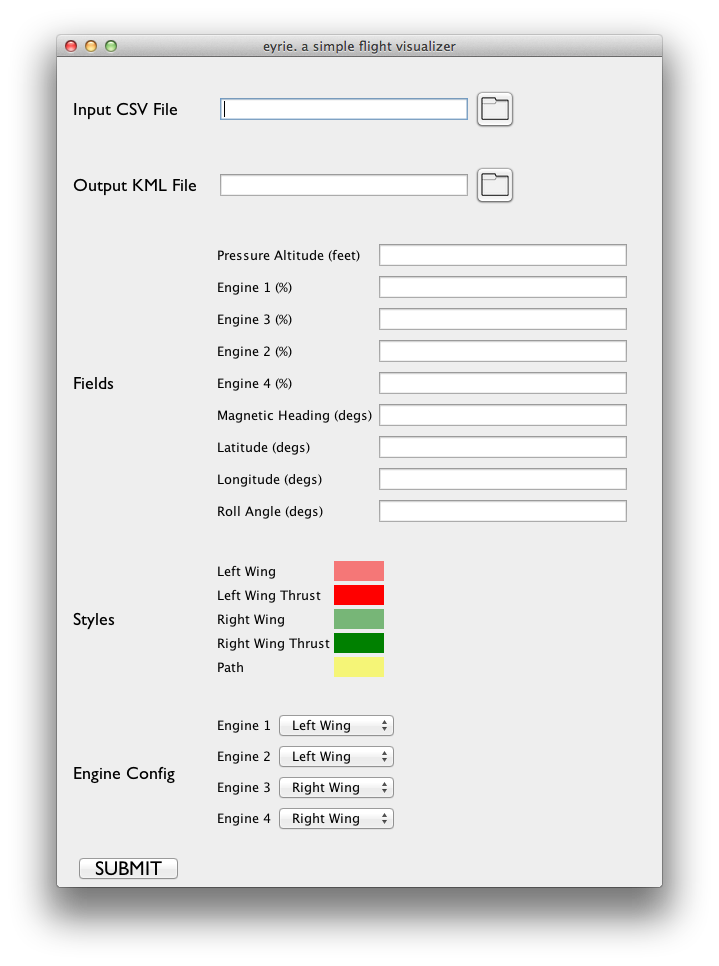
\includegraphics[scale=0.5]{gfx/ui-overview.png}
\caption{An overview of the user interface}
\end{figure}

\subsection{UI Flow}

\begin{enumerate}
\item The user launches the application
\item He/she selects an input csv file. This can be done by either writing the path to the file manually in the text box, or clicking on a button that launches a file picker. As soon as the input file is selected, the application analyses the file's headers and auto fills the fields section. \\
Under the hood, this launches a call to the \lstinline{csv/analyze-headers!} on a separate thread. This is so any processing does not freeze the interface.
\item The user enters the path he/she wants to output to.
\item The user fills up any missing fields, or corrects fields that may have been detected wrong.
\item The user chooses colors for each of the components. Clicking on colored button next to the component name launches a color picker, where the user can choose a new color for that component.
\item Lastly, the user fills up the engine configuration. This specifies which engine is on which wing.
\item The user hits submit.
\item If the file, the user selected was valid
\end{enumerate}

\chapter{Testing Methodology}

Testing for the application took place in 3 main stages. Clojure comes built in with a test framework called clojure.test which was mainly used.

\section{Unit Tests}

Unit tests were particularly important for functions within the \lstinline{math} namespace. The primary reason was because the entire generation component depended on mathematical model being implemented properly. \\

The unit tests also gave an indication of how numerically stable the computations were, especially when dealing with very small distances, or angles that were multiples of $\pi$. As clojure automatically shifted to using java's BigDecimal type when dealing with high precision numbers, thankfully the calculations did not face major numerical instabilities.\\

Unit tests were also used for the parsing stage. This stage was even easier to unit test, primarily because the functionality was relatively simple. The major edge cases I had to consider were cases where input was malformed or corrupted, and to fail gracefully when encountering such cases. \\

However, unit testing the KML generation was not straight forward. The primary reason is that because the application generates a visualization, it is difficult to assess it's validity programmatically, aside from checking for trivial things like coordinates being non empty.

\section{Integration Tests}

Integration tests fell under two main categories:

\begin{enumerate}
\item Testing the parsing and generation components together. Inputs were fed into both components without the UI to test whether these two subsystems integrated properly. Part of this test included checking for correct error handling when given incorrect or corrupt csv inputs. It also included checking for visualizations when several data points were missing. \\
Sadly however, checking the KML output could not be automated and had to be done manually for this stage.
\item Testing all the UI components with the UI flow without coupling them to the application core. Seesaw's selectors made this much easier than I anticipated.
\end{enumerate}

\section{Blackbox Tests}

Testing the entire system was once again something that could not be automated, except for trivial cases, as the system produced a visualization that necessitated manual inspection. \\

To make black box testing easier, I made a list of test cases that I would manually replicate, where I would test for incorrect input files, mistyped field names, and impossible engine configurations, and check whether the UI displayed errors in these cases. \\

One limitation to extensive testing was that I was only given one dataset by AAIB to use for development. Having more datasets would have allowed me to test for more cases.

\chapter{Conclusion}

\section{Summary}

The project started off with what seemed to be a complex problem. The problem was to map raw aircraft attitude data into a form that could be visualised easily. What really helped here though was having a good mental image of what I was expected to render. \\

The next stage was to model this mental image when given the constraints of the output form. As I had chosen KML to render this data, I had to represent whatever images I had in mind, in terms of KML elements. This was intially difficult as I had to visualize simple geometric constructs like lines and polygons in spherical coordinates. \\

However, after researching and finding ways to transform spherical coordinates by distance and bearing, the next steps were easy. \\

Implementation wise, building this system in a language that favored REPL based development, helped me experiment and move quickly with ideas. Furthermore, using well developed DSLs like Hiccup in Clojure made my work significantly easier. \\

\section{Further Work}

Although the project fulfilled the features AAIB requested, it can be improved further. A few features, in my opinion that the current visualisation lacks are:
\begin{itemize}
\item Displaying an aircraft's pitch. This is actualy quite simple to add. For each data point, one could add a line representing the pitch angle, that would run through the aircraft's lateral axis.
\item Displaying an aircraft's yaw. This would be slightly difficult to visualize with the current scheme of things. The difficult would lie in visually differentiating between the yaw and heading, which currenly display on the same axis.
\item Finding a method to overlay data when the user places his mouse over a data point. I actually tried implementing this, but because KML is not designed for complex interactions like mouseover events, this particular feature is not possible with just KML. An alternative could be to launch a description modal when clicking a data point, but with a large number of data points this could look very messy.
\end{itemize}

%----------------------------------------------------------------------------------------
%	THESIS CONTENT - APPENDICES
%----------------------------------------------------------------------------------------

%\appendix

%\part{Appendix} % New part of the thesis for the appendix

%% Appendix A

\chapter{Appendix Test}

%----------------------------------------------------------------------------------------

\lipsum[13-14]

%----------------------------------------------------------------------------------------

\section{Appendix Section Test}
\lipsum[15]

\graffito{More dummy text}
\lipsum[16]

%----------------------------------------------------------------------------------------

\section{Another Appendix Section Test}
\lipsum[17]

\begin{table}
\myfloatalign
\begin{tabularx}{\textwidth}{Xll} \toprule
\tableheadline{labitur bonorum pri no} & \tableheadline{que vista}
& \tableheadline{human} \\ \midrule
fastidii ea ius & germano &  demonstratea \\
suscipit instructior & titulo & personas \\
\midrule
quaestio philosophia & facto & demonstrated \\
\bottomrule
\end{tabularx}
\caption[Autem usu id]{Autem usu id.}
\label{tab:moreexample}
\end{table}

\lipsum[18]

\begin{lstlisting}[float,caption=A floating example]
for i:=maxint to 0 do
begin
{ do nothing }
end;
\end{lstlisting} % Appendix A
%% Appendix X

\chapter{Appendix Title}

%----------------------------------------------------------------------------------------

% Content begins here % Appendix B - empty template

%----------------------------------------------------------------------------------------
%	POST-CONTENT THESIS PAGES
%----------------------------------------------------------------------------------------

\cleardoublepage% Bibliography

\label{app:bibliography} % Reference the bibliography elsewhere with \autoref{app:bibliography}

\manualmark
\markboth{\spacedlowsmallcaps{\bibname}}{\spacedlowsmallcaps{\bibname}}
\refstepcounter{dummy}

\addtocontents{toc}{\protect\vspace{\beforebibskip}} % Place the bibliography slightly below the rest of the document content in the table of contents
\addcontentsline{toc}{chapter}{\tocEntry{\bibname}}

\bibliographystyle{apalike}

\bibliography{Bibliography}
 % Bibliography

%\cleardoublepage% Colophon (a brief description of publication or production notes relevant to the edition)

\pagestyle{empty}

\hfill

\vfill

\pdfbookmark[0]{Colophon}{colophon}

\section*{Colophon}

This document was typeset using the typographical look-and-feel \texttt{classicthesis} developed by Andr\'e Miede. The style was inspired by Robert Bringhurst's seminal book on typography ``\emph{The Elements of Typographic Style}''. \texttt{classicthesis} is available for both \LaTeX\ and \mLyX: 

\begin{center}
\url{http://code.google.com/p/classicthesis/}
\end{center}

\noindent Happy users of \texttt{classicthesis} usually send a real postcard to the author, a collection of postcards received so far is featured here: 

\begin{center}
\url{http://postcards.miede.de/}
\end{center}
 
\bigskip

\noindent\finalVersionString % Colophon

%\cleardoublepage% Declaration

\refstepcounter{dummy}
\pdfbookmark[0]{Declaration}{declaration} % Bookmark name visible in a PDF viewer

\chapter*{Declaration} % Declaration section text

\thispagestyle{empty}

Put your declaration here.
\bigskip
 
\noindent\textit{\myLocation, \myTime}

\smallskip

\begin{flushright}
\begin{tabular}{m{5cm}}
\\ \hline
\centering\myName, \today \\
\end{tabular}
\end{flushright} % Declaration

%----------------------------------------------------------------------------------------

\end{document}
